\chapter{Apêndices}      \label{Apendice}

Além da aplicação nos dispositivos baseados em cristais fotônicos, também foi realizado o procedimento de otimização em dois divisores de potência baseados em grafeno. Na Seção \ref{Aplicacao Divisor}, é mostrada a metodologia e na Seção \ref{Resultado DivPot}, são mostrados os resultados.

\section{APÊNDICE A -- APLICAÇÃO EM DIVISOR DE POTÊNCIA}      \label{Aplicacao Divisor}

Os divisores de potência por três (1x3) baseado em grafeno discutidos em \cite{Dmitriev2021Nonreciprocal} foram submetidos ao procedimento deste trabalho. Como mostrado na Fig. \ref{fig: GrapheneDividers}, o divisor $\mathcal{T}\sigma_{1}$ tem simetria vertical e o divisor $\mathcal{T}\sigma_{2}$, simetria horizontal.

\begin{figure}[H]
    \centering
    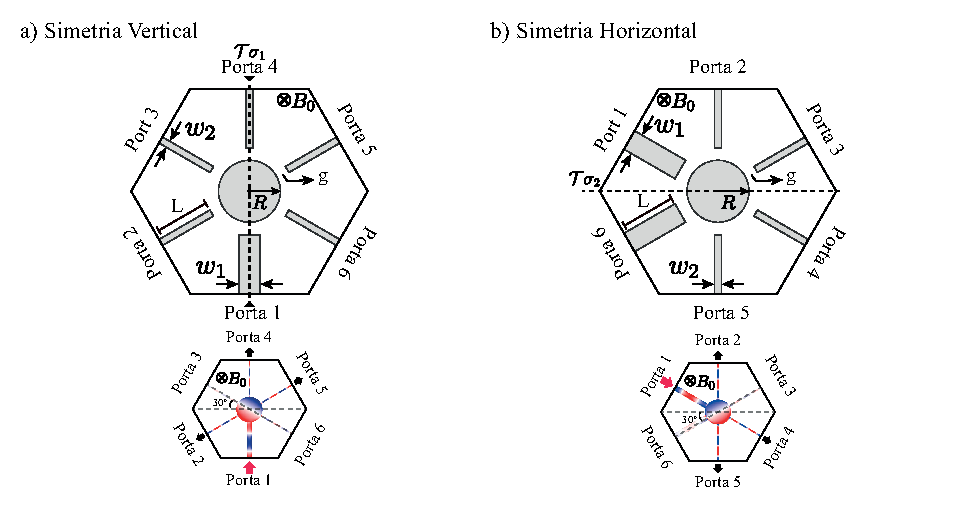
\includegraphics{04-Figuras/GrapheneDividers.eps}
    \caption{Divisores de potência suas respectivas distribuições do campo eletromagnético para excitação na porta 1. a) Divisor $\mathcal{T}\sigma_{1}$. b) Divisor $\mathcal{T}\sigma_{2}$.} \par
    Fonte: Francisco Nobre (2021) (adaptado pelo Autor) \cite{Nobre2021Graphene}.
    \label{fig: GrapheneDividers}
\end{figure}

A geometria de ambos foi parametrizada de modo a respeitar a simetria particular de cada dispositivo. Algumas dessas variáveis são $w_{1}$ e $w_{2}$ (expessura dos guias de onda), $R$ (raio do ressonador), $\otimes B_{0}$ (campo magnético) e $g$ (gap dos guias de onda).


\begin{figure}[H]
	\centering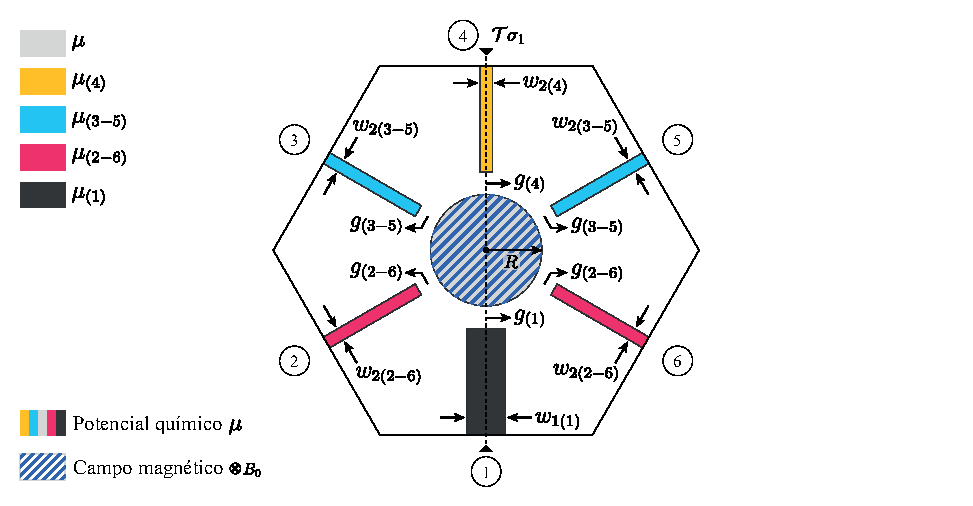
\includegraphics{04-Figuras/VariaveisGeometriaVertical.eps}
	\caption{Variáveis geométricas do divisor vertical $\mathcal{T}\sigma_{1}$.}
    Fonte: do Autor.
	\label{fig: VariaveisGeometriaVertical}
\end{figure}

No total, tanto para $\mathcal{T}\sigma_{1}$ (ver Fig. \ref{fig: VariaveisGeometriaVertical}) quanto para $\mathcal{T}\sigma_{2}$ (ver Fig. \ref{fig: VariaveisGeometriaHorizontal}), foram avaliados $19$ parâmetros geométricos. Assim, o tensor $[Y]$ terá dimensão $i \times 19$ para ambos dispositivos.

\begin{figure}[H]
	\centering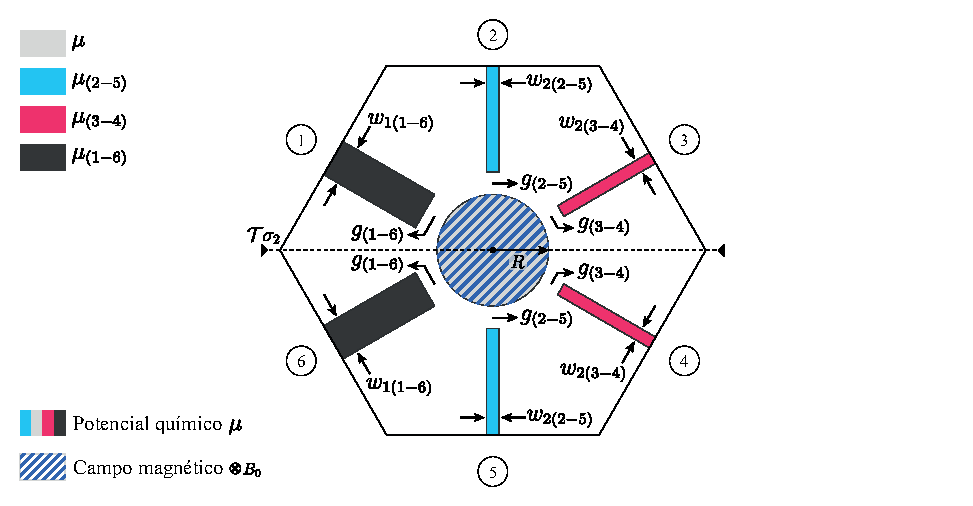
\includegraphics{04-Figuras/VariaveisGeometriaHorizontal.eps}
	\caption{Variáveis geométricas do divisor horizontal $\mathcal{T}\sigma_{2}$.}
    Fonte: do Autor.
	\label{fig: VariaveisGeometriaHorizontal}
\end{figure}

A resposta em frequência é avaliada considerando o desempenho do sinal da \textit{porta 1} para todas as outras (ver \textit{distribuição do campo eletromagnético} na Fig. \ref{fig: GrapheneDividers}). Portanto, $6$ curvas são avaliadas: $S_{11}$, $S_{21}$, $S_{31}$, $S_{41}$, $S_{51}$ e $S_{61}$. Para o divisor $\mathcal{T}\sigma_{1}$, as curvas $S_{21}$, $S_{41}$, $S_{51}$ devem ser maximizadas, pois o sinal deve sair da \textit{porta 1} e se dividir para essas portas, enquanto que as curvas $S_{11}$, $S_{31}$, $S_{61}$ devem ser minimizadas (já que o sinal não deve ser propagado para elas). O mesmo raciocínio se extende para o $\mathcal{T}\sigma_{2}$, sendo as curvas $S_{21}$, $S_{41}$ e $S_{51}$ maximizadas (sinal propagado) e as curvas $S_{11}$, $S_{31}$, $S_{61}$ minimizadas (sinal isolado).


Tanto para o divisor $\mathcal{T}\sigma_{1}$ quanto para o divisor $\mathcal{T}\sigma_{2}$, cada curva da resposta em frequência está discretizada em 51 pontos, portanto, $51 \times 6 = 306$. Isso indica que os tensores $[X]$ e $[Z]$ terão dimensão $i \times 306$ e $1 \times 306$, respectivamente. Desta forma, a rede neural profunda terá $306$ neurônios na camada de entrada e $19$ neurônios na camada de saída para os dois divisores $\mathcal{T}\sigma_{1}$ e $\mathcal{T}\sigma_{2}$.


\subsection{Arquitetura de Rede}

Definido a quantidade de neurônios nas camadas de entrada e saída da rede neural profunda, o próximo passo foi definir a arquitetura de rede. A escolha igual das mesmas quantidades de variáveis de geometria para ambos divisores foi intencional, pois facilita o uso de uma arquitetura para trabalhar ambos dispositivos. Foram desenvolvidas 6 arquiteturas de redes com diversas configurações de neurônios e camadas.

\begin{itemize}
    \item Rede 1: $306 - 150 - 19$
    \item Rede 2: $306 - 200 - 100 - 19$
    \item Rede 3: $306 - 150 - 100 - 50 - 19$
    \item Rede 4: $(51) \parallel \times 6 \rightarrow 306 - 150 - 100 - 50 - 19$
    \item Rede 5: $(51 - 51 - 51) \parallel \times 6 \rightarrow 306 - 150 - 100 - 50 - 19$
    \item Rede 6: $(51 - 51 - 51 - 51 - 51 - 51) \parallel \times 6 \rightarrow 306 - 150 - 100 - 50 - 19$
\end{itemize}

Após a geração do banco de dados inicial $i_{0}$, foi realizado testes de performance das 6 arquiteturas de redes. Primeiramente, foi avaliado o desempenho das três primeiras redes. Foi observado que a \textit{rede 3} obteve o melhor desempenho (isto é, menor erro). Posteriormente, foram geradas mais três arquiteturas de redes (\textit{rede 4}, \textit{rede 5} e \textit{rede 6}), as quais são variações da \textit{rede 3} contendo seis redes de pré-processamento paralelo, variando em $1$, $3$ e $6$ camadas, as quais são conectadas à rede sequencial (\textit{rede 3}) através de uma camada de concatenação\footnote{O símbolo $\rightarrow$ é usado para indicar a concatenação.} (essa arquitetura foi previamente discutida na Fig. \ref{fig: StepNetwork-b}).





\begin{table}[H]
    \centering
    \caption{Performance de cada arquitetura de rede em relação ao banco de dados inicial $i_{0}$ de cada divisor.}
    \begin{tabular}{ccc}
\hline
Rede & \multicolumn{1}{r}{Divisor $\mathcal{T}\sigma_{1}$ (MSE)} & \multicolumn{1}{r}{Divisor $\mathcal{T}\sigma_{2}$ (MSE)} \\ \hline
1    & $3,5325e^{-2}$                                            & $5,4233e^{-2}$                                            \\
2    & $3,1709e^{-2}$                                            & $4,8093e^{-2}$                                            \\
3    & $2,6919e^{-2}$                                            & $3,7429e^{-2}$                                            \\
4    & $2,6228e^{-2}$                                            & $4,1021e^{-2}$                                            \\
5    & $2,3523e^{-2}$                                            & $3,6947e^{-2}$                                            \\
6    & $2,6551e^{-2}$                                            & $4,0931e^{-2}$                                            \\ \hline
\end{tabular}

    \label{tab: ArquiteturaRedeDivisor}

    \vspace{2.5mm}
    Fonte: do Autor.

    \end{table}

Como pode ser conferido na Tabela \ref{tab: ArquiteturaRedeDivisor}, arquitetura de rede 5 foi escolhida para ambos divisores, pois obteve o menor erro (MSE) quando treinada com o banco de dados inicial $i_{0}$.


\subsection{Operação Ideal}

A Fig. \ref{fig: DividerTargetFrequencyResponse} mostra a resposta em frequência ideal designada para ambos divisores, a qual será o objetivo da rede neural. Todas as curvas estão em ressonância na frequência central de operação dos dispositivos. 

\begin{figure}[H]
	\centering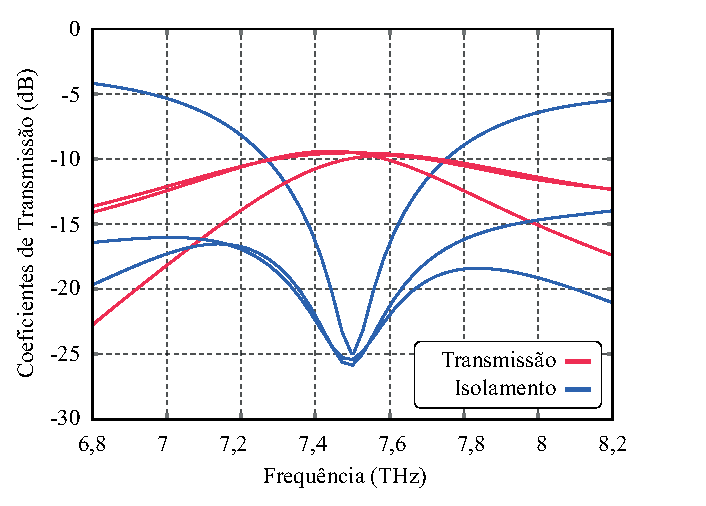
\includegraphics{04-Figuras/DividerTargetFrequencyResponse.eps}
	\caption{Resposta em frequência desejada.}
    Fonte: do Autor.
	\label{fig: DividerTargetFrequencyResponse}
\end{figure}



\subsection{Resultados}      \label{Resultado DivPot}

O objetivo da rede neural profunda foi otimizar e realizar a otimização da geometria do divisor vertical a partir da \textit{resposta em frequência desejada} mostrada na Fig. \ref{fig: DividerTargetFrequencyResponse}. A Fig. \ref{fig: ResultadoVerticalLoop131} mostra a resposta em frequência do divisor $\mathcal{T}\sigma_{1}$ após esse processo de otimização.

\begin{figure}[H]
	\centering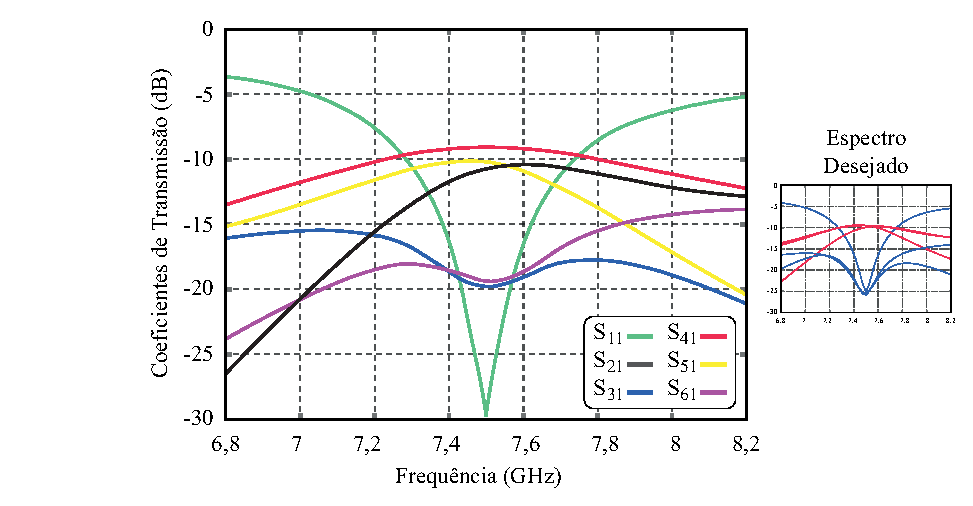
\includegraphics{04-Figuras/ResultadoVerticalLoop131.eps}
	\caption{Resultado da resposta em frequência do divisor vertical $\mathcal{T}\sigma_{1}$.}
    Fonte: Francisco Nobre (2021) (adaptado pelo Autor) \cite{Nobre2021Graphene}.
	\label{fig: ResultadoVerticalLoop131}
\end{figure}

Nota-se que a ressonância ocorre na frequência central do divisor $\mathcal{T}\sigma_{1}$, entretanto, um valor ótimo das curvas de isolamento seria abaixo dos $-20dB$, requisito que ainda não foi respeitado pelas curvas $S_{31}$ e $S_{61}$.

Os parâmetros encontrados pela rede neural (\textit{Valor Otimizado}) para o divisor vertical $\mathcal{T}\sigma_{1}$ podem ser comparados com a situação do dispositivo antes da otimização (\textit{Valor Original}), como mostrado na Tabela \ref{tab: Vertical_Loop_131}.





\begin{table}[H]
    \centering
    \caption{Comparação dos parâmetros do divisor vertical.}
    \begin{tabular}{rccl}
    \hline
\multicolumn{1}{c}{Parâmetros} & Valor Original & Valor Otimizado   & \multicolumn{1}{c}{Descrição}     \\ \hline
$w_{1(1)}$                     & 120nm          & 117,1798nm        & Espessura do guia 1               \\
$w_{2(2-6)}$                   & 28nm           & 28,0957nm         & Espessura dos guia 2 e 6          \\
$C_{(2-6)}$                    & 0$^{\circ}$    & +1,4927$^{\circ}$ & Contorno dos guias 2 e 6          \\
$w_{2(3-5)}$                   & 28nm           & 32,8879nm         & Espessura dos guia 3 e 5          \\
$C_{(3-5)}$                    & 0$^{\circ}$    & +4,8879$^{\circ}$ & Contorno dos guias 3 e 5          \\
$w_{2(4)}$                     & 28nm           & 28,5929nm         & Espessura do guia 4               \\
$\mu$                          & 0,15eV         & 0,1571eV          & Potencial químico do ressonador   \\
$\mu_{(1)}$                    & 0,15eV         & 0,1657eV          & Potencial químico do guia 1       \\
$\mu_{(2-6)}$                  & 0,15eV         & 0,1397eV          & Potencial químico dos guias 2 e 6 \\
$\mu_{(3-5)}$                  & 0,15eV         & 0,1631eV          & Potencial químico dos guias 3 e 5 \\
$\mu_{(4)}$                    & 0,15eV         & 0,1585eV          & Potencial químico do guia 4       \\
$B_{0}$                        & 0,29T          & 0,2079T           & Campo magnético                   \\
$R$                            & 320nm          & 328,8418nm        & Raio do ressonador                \\
$g_{(1)}$                      & 2,5nm          & 2,3263nm          & Gap do guia 1                     \\
$g_{(2-6)}$                    & 2,5nm          & 1,7391nm          & Gap dos guias 2 e 6               \\
$g_{(3-5)}$                    & 2,5nm          & 3,6179nm          & Gap dos guias 3 e 5               \\
$g_{(4)}$                      & 2,5nm          & 4,4295nm          & Gap do guia 4                     \\ \hline
\end{tabular}

    \label{tab: Vertical_Loop_131}

    \vspace{2.5mm}
    Fonte: Francisco Nobre (2021) \cite{Nobre2021Graphene}.

    \end{table}

A resposta em frequência do divisor de simetria horizontal $\mathcal{T}\sigma_{2}$ após o procedimento de otimização está ilustrada na Fig. \ref{fig: ResultadoHorizontalLoop267}.

\begin{figure}[H]
	\centering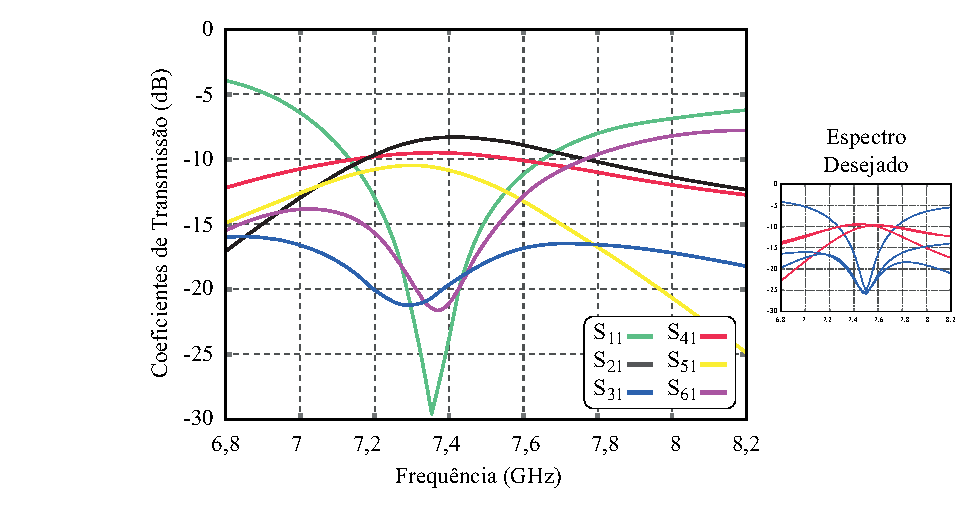
\includegraphics{04-Figuras/ResultadoHorizontalLoop267.eps}
	\caption{Resultado da resposta em frequência do divisor horizontal $\mathcal{T}\sigma_{2}$.}
    Fonte: Francisco Nobre (2021) (adaptado pelo Autor) \cite{Nobre2021Graphene}.
	\label{fig: ResultadoHorizontalLoop267}
\end{figure}

Nota-se que o procedimento ainda não foi satisfatório, pois as curvas não estão em ressonância na frequência central de operação do divisor $\mathcal{T}\sigma_{2}$. No total, foram realizados $215$ \textit{Loops} para o divisor $\mathcal{T}\sigma_{1}$ e $634$ \textit{Loops} para o divisor $\mathcal{T}\sigma_{2}$, como mostrado na Tabela \ref{tab: MSEDivisor}.





\begin{table}[H]
    \centering
    \caption{Comparação do desempenho de otimização dos divisores.}
    \begin{tabular}{rccl}
    \hline
\multicolumn{1}{c}{Dispositivo} & Loop & MSE               & \multicolumn{1}{c}{Descrição} \\ \hline
$\mathcal{T}\sigma_{1}$         & 215  & 0,007188          & Divisor Vertical              \\
$\mathcal{T}\sigma_{2}$         & 634  & 0,038134          & Divisor Horizontal            \\ \hline
\end{tabular}

    \label{tab: MSEDivisor}

    \vspace{2.5mm}
    Fonte: do Autor.

    \end{table}


\newpage
\section{APÊNDICE B -- CRISTAL FOTÔNICO: PARÂMETROS GERAIS}      \label{PhC}

Esta Seção do Apêndice detalha a geometria dos dispositivos baseados em cristal fotônico e as características de projeto da rede neural profunda implementada.

\subsection{Características da Geometria}

A estrutura geométrica dos dispositivos baseados em cristais fotônicos está apresentada na Fig. \ref{fig: PhCParametrization}. Ela é composta por cilindros em uma estrutura periódica, cuja a constante de rede $a$ é de 0,12 mm. Cada cilindro tem o raio de $0,2a$ mm e posição (centro do cilindro em coordenadas cartesianas $(x, y)$) em valores discretos da constante de rede.

\begin{figure}[H]
    \centering
    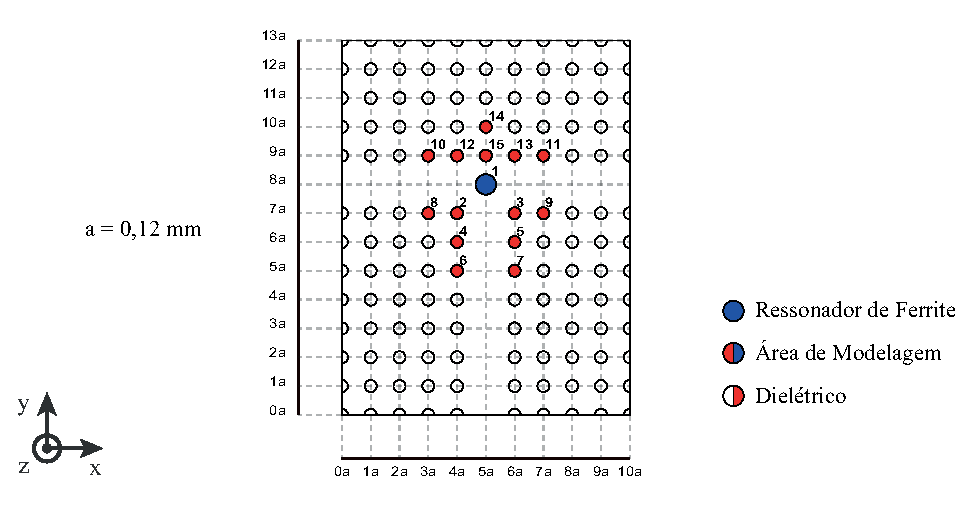
\includegraphics{04-Figuras/PhCParametrization.eps}
    \caption{Parametrização da geometria base do cristal fotônico.} \par
    Fonte: do Autor.
    \label{fig: PhCParametrization}
\end{figure}

A ferrite, localizada no centro da \textit{junção-T}, tem raio específico para cada dispositivo. Para o dispositivo de ressonância dipolo, o raio da ferrite é de $0,2a$ mm, enquanto que para o dispositivo de ressonância quadrupolo, o raio da ferrite é de $0,4a$ mm. A ferrite posta na cavidade ressonante é magnetizada por um campo magnético externo e irá apresentar \textit{dois} ou \textit{quatro} polos, a depender do raio que a ferrite apresentar.

A Tabela \ref{tab: DipoloOtimizado} mostra os valores de geometria do dispositivo dipolo em milímetros. O \textit{valor original} refere-se à geometria base e o \textit{valor otimizado} à geometria otimizada, como mostrado na Fig. \ref{fig: PhCGeometryOptimization}.a) e \ref{fig: PhCGeometryOptimization}.b), respectivamente.





\begin{table}[H]
    \centering
    \caption{Parâmetros otimizados do circulador dipolo.}
\begin{tabular}{ccccc}
\hline
         & \multicolumn{2}{c}{Valor Original} & \multicolumn{2}{c}{Valor Otimizado}              \\ \hline
Cilindro & Centro (x, y)        & Raio        & Centro (x, y)      & Raio                        \\ \hline
1        & (5a, 8a)             & 0,2a        & (5a, 7,438a)       & \multicolumn{1}{l}{0,2854a} \\
2        & (4a, 7a)             & 0,2a        & (4,9399a, 6,9244a) & \multicolumn{1}{l}{0,2228a} \\
3        & (6a, 7a)             & 0,2a        & (6,061a, 6,9244a)  & 0,2228a                     \\
4        & (4a, 6a)             & 0,2a        & (4,9518a, 6,1150a) & 0,2060a                     \\
5        & (6a, 6a)             & 0,2a        & (6,0482a, 6,1150a) & 0,2060a                     \\
6        & (4a, 5a)             & 0,2a        & (4,996a, 5,1150a)  & 0,2a                        \\
7        & (6a, 5a)             & 0,2a        & (6,0996a, 5,1150a) & 0,2a                        \\
8        & (3a, 7a)             & 0,2a        & (3a, 7a)           & 0,2a                        \\
9        & (7a, 7a)             & 0,2a        & (7a, 7a)           & 0,2a                        \\
10       & (3a, 9a)             & 0,2a        & (3a, 9,0384a)      & 0,2023a                     \\
11       & (7a, 9a)             & 0,2a        & (7a, 9,0384a)      & 0,2023a                     \\
12       & (4a, 9a)             & 0,2a        & (4,0786a, 8,8963a) & 0,2012a                     \\
13       & (6a, 9a)             & 0,2a        & (5,9214a, 8,8963a) & 0,2012a                     \\
14       & (5a, 10a)            & 0,2a        & (5a, 9,2305a)      & 0,0953a                     \\
15       & (5a, 9a)             & 0,2a        & (5a, 9,9823a)      & 0,2a                        \\ \hline
\end{tabular}

    \label{tab: DipoloOtimizado}

    \vspace{2.5mm}
    Fonte: do Autor.

\end{table}

Na Tabela \ref{tab: QuadrupoloOtimizado}, o \textit{valor original} também refere-se à geometria base e o \textit{valor otimizado} à geometria otimizada para o circulador quadrupolo, como mostrado na Fig. \ref{fig: PhCGeometryOptimization}.a) e \ref{fig: PhCGeometryOptimization}.c), respectivamente.





\begin{table}[H]
    \centering
    \caption{Parâmetros otimizados do circulador quadrupolo.}
\begin{tabular}{ccccc}
\hline
         & \multicolumn{2}{c}{Valor Original} & \multicolumn{2}{c}{Valor Otimizado}                         \\ \hline
Cilindro & Centro (x, y)        & Raio        & Centro (x, y)              & Raio                           \\ \hline
1        & (5a, 8a)             & 0,4a        & (5a, 7,68491a)             & \multicolumn{1}{l}{0,461478a}  \\
2        & (4a, 7a)             & 0,2a        & (3,849055a, 6,9923255a)    & \multicolumn{1}{l}{0,0637046a} \\
3        & (6a, 7a)             & 0,2a        & (6,150944a, 6,9923255a)    & \multicolumn{1}{l}{0,0637046a} \\
4        & (4a, 6a)             & 0,2a        & (3,983052a, 5,8950494a)    & 0,20221a                       \\
5        & (6a, 6a)             & 0,2a        & (6,016947a, 5,8950494a)    & 0,20221a                       \\
6        & (4a, 5a)             & 0,2a        & (4,085462a, 4,780541082a)  & 0,39467277a                    \\
7        & (6a, 5a)             & 0,2a        & (5,914537a, 4,780541082a)  & 0,39467277a                    \\
8        & (3a, 7a)             & 0,2a        & (2,908861a, 6,84256803a)   & 0,19825571a                    \\
9        & (7a, 7a)             & 0,2a        & (7,091138a, 6,84256803a)   & 0,19825571a                    \\
10       & (3a, 9a)             & 0,2a        & (3,100644a, 9,26410546a)   & 0,19975595a                    \\
11       & (7a, 9a)             & 0,2a        & (6,89935599a, 9,26410546a) & 0,19975595a                    \\
12       & (4a, 9a)             & 0,2a        & (4,05160417a, 9,18938524a) & 0,20172808a                    \\
13       & (6a, 9a)             & 0,2a        & (5,94839582a, 9,18938524a) & 0,20172808a                    \\
14       & (5a, 10a)            & 0,2a        & (5a, 10,10774003a)         & 0,20051608a                    \\
15       & (5a, 9a)             & 0,2a        & (5a, 9,58835201a)          & 0,10690515a                    \\ \hline
\end{tabular}

    \label{tab: QuadrupoloOtimizado}

    \vspace{2.5mm}
    Fonte: do Autor.

\end{table}




\subsection{Hiperparâmetros da Rede Neural}

A rede neural profunda usada para ambos dispositivos baseados em cristais fotônicos tem os seus hiperparâmetros mostrados na Tabela \ref{tab: Hiperparametros}.





\begin{table}[H]
    \centering
    \caption{Hiperparâmetros da rede neural.}
\begin{tabular}{cc}
\hline
Hiperparâmetro     & Atributo                  \\ \hline
Otimizador         & ADAM; $\eta = 0,001$      \\
Função Custo       & MSE                       \\
Função de Ativação & LeakyReLU; $\alpha = 0,3$ \\
Batch Size         & 100                       \\
Épocas             & 20000                     \\ \hline
\end{tabular}

    \label{tab: Hiperparametros}

    \vspace{2.5mm}
    Fonte: do Autor.

\end{table}

Assim, $\eta$ refere-se a taxa de aprendizazem do otimizador ADAM, enquanto que $\alpha$ refere-se ao coeficiente de inclinação negativo da função de ativação LeakyReLU.

A Tabela \ref{tab: DivBancoDeDados} mostra a divisão percentual do danco de dados em \textit{treino}, \textit{validação} e \textit{teste}.





\begin{table}[H]
    \centering
    \caption{Divisão do banco de dados.}
\begin{tabular}{cc}
\hline
Composição & Atributo \\ \hline
Treino     & 80\%     \\
Validação  & 10\%     \\
Teste      & 10\%     \\ \hline
\end{tabular}

    \label{tab: DivBancoDeDados}

    \vspace{2.5mm}
    Fonte: do Autor.

\end{table}


\subsection{Configurações da Máquina}

As configurações do computador onde todo o procedimento de otimização foi rodado, estão mostradas na Tabela \ref{tab: ConfigPC}.





\begin{table}[H]
    \centering
    \caption{Configurações do computador.}
\begin{tabular}{cc}
\hline
Característica        & Atributo               \\ \hline
CPU                   & Intel Core i5-3210M    \\
GPU                   & NVIDIA GeForce GT-630M \\
Memória               & 8 GB                   \\
Armazenamento         & SSD 250 GB             \\
Sistema Operacional   & Windows 10             \\
COMSOL                & Versão 5.5             \\
MATLAB                & Versão R2020B          \\
Tempo 1               & 15 minutos             \\
Tempo 2               & 20 minutos             \\
Tempo 3               & 3 semanas - 5 semanas  \\ \hline
\end{tabular}

    \label{tab: ConfigPC}

    \vspace{2.5mm}
    Fonte: do Autor.

\end{table}

Desta maneira, o \textit{Tempo 1} refere-se ao tempo demandado para o computador especificado rodar uma simulação do COMSOL, enquanto que o \textit{Tempo 2} refere-se ao tempo necessário para treinar a rede neural. O \textit{Tempo 3} foi o tempo total gasto para todo o processo de otimização e modelagem inversa apresentado neste trabalho. O dispositivo circulador de ressonância dipolo demandou 3 semanas, enquanto que o dispositivo circulador de ressonância quadrupolo demandou 5 semanas. É válido ressaltar que o \textit{Tempo 3} não ocorreu de forma initerrupta.